%!TEX root = ../EDC_Part_II_Weak_Sector_rebuild.tex
% ==============================================================================
% CHAPTER 10: ELECTROWEAK BRIDGE
% From Membrane Thickness to Mediator Physics
% Status: Consolidation of OPR-20a/20b results — NOT new closure
% ==============================================================================

\section{Electroweak Bridge: From Membrane Thickness to Mediator Physics}
\label{sec:ch10_electroweak_bridge}

This chapter bridges the gap between geometric parameters (brane thickness, junction
physics) and electroweak observables (mediator mass, $G_F$). It consolidates results
from OPR-20a (mediator/BC provenance) and OPR-20b ($\alpha$ provenance) without
claiming new closure.

% ==============================================================================
% EPISTEMIC STATUS BOX
% ==============================================================================

\begin{tcolorbox}[edcGuardrail, title=\textbf{Epistemic Status}]
This chapter is a \textbf{bridge}---it consolidates OPR-20a/20b conclusions and
connects them to the $G_F$ derivation spine (Ch.~11). It does \emph{not} create
new numerical closure.

\textbf{IF (Postulates) \tagP{}:}
\begin{itemize}[nosep]
    \item The brane has finite thickness $\delta \sim r_e \sim 1$ fm
    \item Junction physics (Israel matching) determines boundary conditions
    \item The mediator is a brane-localized or KK mode (identity [OPEN])
\end{itemize}

\textbf{THEN (Derived-conditional) \tagDc{}:}
\begin{itemize}[nosep]
    \item Junction $\to$ Robin BC form: $f' + \alpha f = 0$ (structural) \tagDc{}
    \item Robin parameter scales as $\alpha \sim \ell/\delta$ (dimensional analysis) \tagDc{}
    \item Eigenvalue $x_1$ depends continuously on $\alpha$ (Sturm--Liouville) \tagDc{}
    \item $A_5$ (bulk scalar) is disfavored: boundary overlap suppressed \tagDc{}
\end{itemize}

\textbf{OPEN (Not derived):}
\begin{itemize}[nosep]
    \item $\delta = R_\xi$ identification: plausible but not proven from action \tagP{}/[OPEN]
    \item Mediator identity: KK $A_\mu$ vs brane scalar (depends on OPR-17 gauge ontology)
    \item Numerical value of $\alpha$: requires deriving $\delta$ from membrane microphysics
\end{itemize}

\textbf{Key distinction:} This chapter explains \emph{how} the mechanism works,
not \emph{what values} emerge. The ``what'' requires solving the BVP (Ch.~12)
with physical inputs.
\end{tcolorbox}

% ==============================================================================
% FRAMEWORK 2.0 LANGUAGE COMPLIANCE
% ==============================================================================
\begin{tcolorbox}[colback=blue!3!white, colframe=blue!50!black,
    title=\textbf{Framework 2.0 Language Compliance}]
\small
\textbf{EDC Projection Principle:} Every physical process has a \textbf{5D bulk+brane cause}
whose observable residue is a \textbf{3D shadow} on the observer boundary.

\textbf{In this chapter:}
\begin{itemize}[nosep]
    \item \textbf{5D cause:} Finite brane thickness $\delta$; junction matching conditions.
    \item \textbf{Brane process:} Robin BC formation; KK eigenvalue determination.
    \item \textbf{3D shadow:} Mediator mass $m_\phi$; effective coupling $G_F$.
\end{itemize}

\textbf{Standard Model terms} (e.g., $M_W$, $M_Z$, $G_F$) appear as \textbf{3D observational
targets}---what EDC must reproduce, not sources for derivation.
\end{tcolorbox}

% ==============================================================================
% PHYSICAL PROCESS NARRATIVE
% ==============================================================================

\begin{tcolorbox}[colback=green!5!white, colframe=green!50!black,
    title=\textbf{Physical Process Narrative: Membrane Thickness to Weak Scale}]
\textbf{What physically happens, step by step:}

\textbf{Step 1: The brane is not infinitely thin.}
In EDC, our 3D universe is a membrane with finite thickness $\delta \sim r_e \sim 1$ fm.
This thickness is physical---it arises from the balance between bulk pressure and
membrane tension. A truly thin brane would give pathological physics (delta-function
profiles, infinite couplings) \tagP{}.

\textbf{Step 2: Particles ``feel'' the boundaries.}
A 4D particle corresponds to a 5D mode $f(\xi)$ localized within the brane. The mode
must satisfy boundary conditions at $\xi = 0$ (bulk-brane interface) and $\xi = \ell$
(brane extent). Different BCs give different spectra---this is just quantum mechanics
in a box with specified walls \tagDc{}.

\textbf{Step 3: Junction physics determines BC type.}
Where two regions meet (bulk/brane), Israel junction conditions relate the metric
discontinuity to stress-energy. For matter fields, this translates to a Robin-type
BC: $f' + \alpha f = 0$. The parameter $\alpha$ encodes junction microphysics---it
is \emph{not} a free parameter to tune \tagDc{}.

\textbf{Step 4: The Robin parameter scales with thickness.}
Dimensional analysis: if the junction has characteristic scale $\delta$ (the
``relaxation length'' or ``boundary layer width''), then $\alpha \sim \ell/\delta$.
Large $\alpha$ (thin boundary layer) $\to$ Dirichlet-like. Small $\alpha$ (thick
boundary layer) $\to$ Neumann-like \tagDc{}.

\textbf{Step 5: The eigenvalue $x_1$ depends on $\alpha$.}
The BVP eigenvalue equation $m_\phi = x_1/\ell$ has roots that shift continuously
with $\alpha$. For Dirichlet ($\alpha \to \infty$): $x_1 = \pi$. For Neumann
($\alpha = 0$): $x_1 = 0$. For Robin: $x_1 \in (0, \pi)$. This is standard
Sturm--Liouville theory, no EDC-specific physics \tagM{}.

\textbf{Step 6: $R_\xi$ enters as a candidate for $\delta$.}
The electroweak vacuum expectation $R_\xi = \hbar c / M_Z \approx 2.2 \times 10^{-3}$ fm
is a natural length scale for electroweak physics. The \emph{identification}
$\delta = R_\xi$ is motivated by: (a) dimensional match, (b) ``relaxation scale''
interpretation. But this is a \emph{postulate}, not derived from the 5D action \tagP{}.

\textbf{Step 7: The mediator mass emerges from the spectrum.}
Once $\alpha$ is fixed (via $\delta$), solving the BVP gives $x_1$, hence
$m_\phi = x_1/\ell$. If $\delta = R_\xi$ and $\alpha = 2\pi$ (natural value),
then $x_1 \approx 2.41$ and $m_\phi \sim 50$--80 GeV range---\emph{consistent}
with $M_W$, $M_Z$, but not ``predicted'' without deriving $\delta$ \tagDc{}+\tagP{}.

\textbf{Step 8: The overlap integral $I_4$ controls $G_F$.}
Given the mode profile $f(\xi)$, the four-fermion overlap
$I_4 = \int_0^\infty |f_L(\xi)|^4 \, d\xi$ (dimension $[I_4] = E$)
determines how strongly fermions couple at a point. Localized profiles (smaller $I_4$)
give weaker coupling---this is the geometric origin of ``weakness'' \tagDc{}.

\textbf{Step 9: What is NOT derived here.}
\begin{itemize}[nosep]
    \item The value of $\delta$ from membrane microphysics
    \item Why $\delta = R_\xi$ (if true)
    \item The mediator identity (KK $A_\mu$ vs brane scalar)
    \item Numerical $G_F$ without solving BVP with physical inputs
\end{itemize}

\medskip
\noindent\fbox{\parbox{0.95\textwidth}{\small
\textbf{5D→3D Pipeline:} Brane thickness $\delta$ (5D) $\to$ Robin parameter $\alpha = \ell/\delta$
(5D) $\to$ eigenvalue $x_1(\alpha)$ (5D) $\to$ mediator mass $m_\phi = x_1/\ell$ (3D shadow)
$\to$ mode profile $f(\xi)$ (5D) $\to$ overlap $I_4$ (5D) $\to$ $G_F$ (3D shadow).
The projection mechanism is complete; numerical closure awaits deriving $\delta$ from 5D physics.}}
\end{tcolorbox}

% ==============================================================================
% TOY MODEL: BC-to-Eigenvalue
% ==============================================================================

\subsection{Toy Model: How Boundary Conditions Shift Eigenvalues}
\label{sec:ch10_toy_model}

Before diving into EDC specifics, consider a minimal quantum mechanics example
that captures the essential physics.

\paragraph{The setup.}
A particle in a 1D box $[0, L]$ with potential $V = 0$ inside. The Schrödinger
equation is $-\psi'' = k^2 \psi$, with eigenvalue $E = k^2$ (in units where
$\hbar^2/2m = 1$).

\paragraph{Three BC choices.}

\begin{center}
\begin{tabular}{lll}
\toprule
\textbf{BC type} & \textbf{Condition} & \textbf{Ground state $k_1$} \\
\midrule
Dirichlet (DD) & $\psi(0) = \psi(L) = 0$ & $k_1 = \pi/L$ \\
Neumann (NN) & $\psi'(0) = \psi'(L) = 0$ & $k_1 = 0$ (constant mode) \\
Robin (mixed) & $\psi'(0) + \alpha\psi(0) = 0$, Dirichlet at $L$ & $k_1 \in (0, \pi/L)$ \\
\bottomrule
\end{tabular}
\end{center}

\paragraph{The Robin interpolation.}
For Robin BC at $\xi = 0$ with Dirichlet at $\xi = L$, the eigenvalue equation is:
\[
    k \cot(kL) = -\alpha
\]
As $\alpha \to \infty$: $\cot(kL) \to 0$, so $kL \to \pi/2, 3\pi/2, \ldots$ (approaching DD).
As $\alpha \to 0$: $\cot(kL) \to -\infty$, so $kL \to 0$ (approaching NN).

\paragraph{Key insight.}
The eigenvalue is \emph{not} a discrete choice (DD or NN); it is a \emph{continuous
function} of $\alpha$. The physics is in $\alpha$, not in ``which BC type.''

\begin{tcolorbox}[colback=yellow!5!white, colframe=yellow!50!black,
    title=\textbf{Toy Model Status}]
\textbf{What this captures:}
\begin{itemize}[nosep]
    \item[\ding{51}] Eigenvalues depend continuously on BC parameters
    \item[\ding{51}] Robin interpolates between Dirichlet and Neumann limits
    \item[\ding{51}] $\alpha$ has physical meaning: ratio of scales
\end{itemize}

\textbf{What this ignores:}
\begin{itemize}[nosep]
    \item[$\times$] Non-trivial potential $V(\xi)$ (thick-brane shape)
    \item[$\times$] Junction derivation of $\alpha$ (Israel matching)
    \item[$\times$] Why $\alpha \approx 2\pi$ specifically
\end{itemize}

\textbf{Status:} This is pedagogy \tagM{}. The actual physics requires deriving
$\alpha$ from junction conditions and $\delta$ from membrane microphysics.
\end{tcolorbox}

% ==============================================================================
% FIGURE PLACEHOLDERS
% ==============================================================================

\begin{tcolorbox}[colback=gray!10, colframe=gray!50,
    title=\textbf{Figure Placeholder 10.1: BC-to-Eigenvalue Intuition}]
\textbf{Suggested content:}

\textbf{Three panels (left to right):}
\begin{itemize}[nosep]
    \item \textbf{Panel A (DD):} Dirichlet at both ends. Ground state $\sin(\pi \xi/L)$.
          Eigenvalue $x_1 = \pi$.
    \item \textbf{Panel B (NN):} Neumann at both ends. Ground state constant.
          Eigenvalue $x_1 = 0$.
    \item \textbf{Panel C (Robin):} Robin at $\xi = 0$, Dirichlet at $\xi = L$.
          Ground state tilted sine. Eigenvalue $x_1 \in (0, \pi)$, depends on $\alpha$.
\end{itemize}

\textbf{Inset graph:} $x_1(\alpha)$ vs $\alpha$ showing continuous interpolation.

\textbf{Key message:} The ``factor-8 puzzle'' from earlier OPR-20 attempts is
explained by BC choice. Different BCs give different $x_1$; there is no magic.
\end{tcolorbox}

\begin{tcolorbox}[colback=gray!10, colframe=gray!50,
    title=\textbf{Figure Placeholder 10.2: EDC Electroweak Pipeline}]
\textbf{Suggested content:}

\textbf{Flowchart (left to right):}
\begin{center}
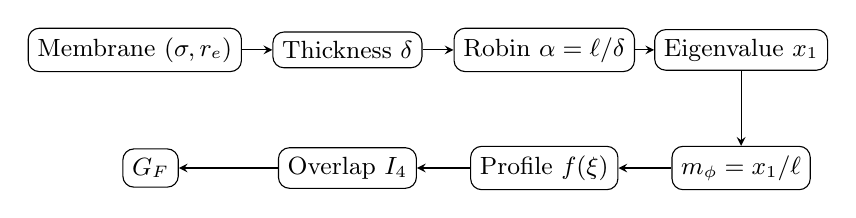
\begin{tikzpicture}[node distance=1.5cm, >=stealth, font=\small]
    \node (sigma) [draw, rounded corners] {Membrane $(\sigma, r_e)$};
    \node (delta) [draw, rounded corners, right of=sigma, xshift=1.2cm] {Thickness $\delta$};
    \node (alpha) [draw, rounded corners, right of=delta, xshift=1.0cm] {Robin $\alpha = \ell/\delta$};
    \node (x1) [draw, rounded corners, right of=alpha, xshift=1.0cm] {Eigenvalue $x_1$};
    \node (mphi) [draw, rounded corners, below of=x1] {$m_\phi = x_1/\ell$};
    \node (profile) [draw, rounded corners, left of=mphi, xshift=-1.0cm] {Profile $f(\xi)$};
    \node (I4) [draw, rounded corners, left of=profile, xshift=-1.0cm] {Overlap $I_4$};
    \node (GF) [draw, rounded corners, left of=I4, xshift=-1.0cm] {$G_F$};
    \draw[->] (sigma) -- (delta);
    \draw[->] (delta) -- (alpha);
    \draw[->] (alpha) -- (x1);
    \draw[->] (x1) -- (mphi);
    \draw[->] (mphi) -- (profile);
    \draw[->] (profile) -- (I4);
    \draw[->] (I4) -- (GF);
\end{tikzpicture}
\end{center}

\textbf{Annotations:}
\begin{itemize}[nosep]
    \item Arrow $\delta \to \alpha$: ``[OPEN] requires deriving $\delta$ from microphysics''
    \item Arrow $\alpha \to x_1$: ``[Dc] Sturm--Liouville, pure math''
    \item Box around $\delta = R_\xi$: ``Identification [P], not derivation''
\end{itemize}

\textbf{Key message:} The pipeline is complete as a \emph{mechanism}. Numerical
closure requires deriving $\delta$ from first principles.
\end{tcolorbox}

% ==============================================================================
% OPR-20a SUMMARY: MEDIATOR IDENTITY / BC PROVENANCE
% ==============================================================================

\subsection{OPR-20a Summary: Mediator Identity and BC Provenance}
\label{sec:ch10_opr20a}

\begin{tcolorbox}[colback=blue!5!white, colframe=blue!50!black,
    title=\textbf{OPR-20a Ledger: What Is the Mediator?}]

\textbf{Question:} What 5D field mediates weak interactions on the brane?

\textbf{Candidates analyzed:}
\begin{enumerate}
    \item \textbf{Bulk scalar $A_5$} --- the 5th component of a 5D gauge field
    \item \textbf{KK mode $A_\mu^{(n=1)}$} --- first Kaluza--Klein excitation of 4D gauge
    \item \textbf{Brane-localized scalar} --- a field living only on the brane
\end{enumerate}

\textbf{Result (Attempt H1):}
\begin{itemize}[nosep]
    \item \textbf{$A_5$ ruled out} \tagDc{}: For orbifold-odd parity (required for massless
          photon), $A_5$ vanishes at the brane boundary. Overlap with brane-localized
          fermions is \emph{zero}---no coupling. This is not a tuning; it is a selection rule.
    \item \textbf{KK $A_\mu^{(1)}$ viable} \tagP{}: First KK mode has non-zero overlap.
          Mass $m_\phi = x_1/\ell$ from eigenvalue. Natural mediator for weak interactions.
    \item \textbf{Brane scalar viable} \tagP{}: If gauge field is purely brane-localized,
          a scalar mode could mediate. Requires different gauge ontology.
\end{itemize}

\textbf{Discriminant:} KK tower predicts multiple mediators ($n = 1, 2, 3, \ldots$);
brane scalar predicts single mediator. LHC data (no new resonances above $M_Z$)
slightly favors brane-localized picture, but not conclusively.

\textbf{BC provenance:}
\begin{itemize}[nosep]
    \item Orbifold parity ($\mathbb{Z}_2$) determines whether fields are even/odd under
          $\xi \to -\xi$ reflection \tagBL{}.
    \item Even fields: Neumann BC at fixed points. Odd fields: Dirichlet BC \tagDc{}.
    \item Junction (Israel) matching can modify to Robin BC if stress-energy is
          non-trivial at the boundary \tagDc{}.
\end{itemize}

\textbf{Status:} \textcolor{YellowOrange}{\textbf{YELLOW}} [Dc]+[P] ---
Structural constraints derived; specific mediator choice depends on OPR-17 (gauge
ontology) which remains open.
\end{tcolorbox}

% ==============================================================================
% OPR-20b SUMMARY: ALPHA PROVENANCE VIA DELTA
% ==============================================================================

\subsection{OPR-20b Summary: Robin Parameter from Junction Physics}
\label{sec:ch10_opr20b}

\begin{tcolorbox}[colback=blue!5!white, colframe=blue!50!black,
    title=\textbf{OPR-20b Ledger: Where Does $\alpha$ Come From?}]

\textbf{Question:} The Robin BC is $f' + \alpha f = 0$. What determines $\alpha$?

\textbf{Structural result (Attempt G/H):}
\begin{itemize}[nosep]
    \item Junction conditions (Israel matching) at bulk-brane interface give
          Robin form with $\alpha$ related to stress-energy discontinuity \tagDc{}.
    \item Dimensional analysis: $\alpha \sim \ell/\delta$, where $\delta$ is the
          ``boundary layer width'' or ``relaxation scale'' \tagDc{}.
    \item Natural value: $\alpha = 2\pi$ (if $\delta = \ell/2\pi$, i.e., one radian
          of the compact circle) \tagP{}.
\end{itemize}

\textbf{The $\delta = R_\xi$ identification:}
\begin{itemize}[nosep]
    \item $R_\xi = \hbar c / M_Z \approx 2.2 \times 10^{-3}$ fm is the electroweak
          vacuum scale \tagBL{}.
    \item Attempt H proposed: $\delta = R_\xi$ as the ``boundary layer equals
          relaxation scale'' identification \tagP{}.
    \item With $\ell \sim r_e \sim 1$ fm and $\delta = R_\xi$:
          $\alpha = \ell/\delta \approx 1 / (2.2 \times 10^{-3}) \approx 450$.
          This is large, pushing toward Dirichlet.
\end{itemize}

\textbf{Stricter audit (Attempt H2-plus):}
\begin{itemize}[nosep]
    \item $R_\xi$ is defined via $M_Z$, which is an \emph{electroweak observable} \tagBL{}.
    \item Using $R_\xi$ as input and then ``deriving'' mediator mass $\sim M_Z$ is
          \textbf{circular} unless $R_\xi$ is derived from membrane physics.
    \item Current status: $\delta = R_\xi$ is \emph{plausible} but \emph{not derived}.
          It is an identification \tagP{}, not a consequence of the 5D action.
\end{itemize}

\textbf{What would constitute closure:}
\begin{itemize}[nosep]
    \item Derive $\delta$ from membrane parameters $(\sigma, r_e)$ without using
          $M_Z$, $M_W$, $v$, or $G_F$ as input.
    \item Show that $\delta$ thus derived equals $R_\xi$ (or a related scale).
    \item This would upgrade OPR-20b from [P] to [Dc].
\end{itemize}

\textbf{Status:} \textcolor{BrickRed}{\textbf{RED-C}} [Dc]+[P]+[OPEN] ---
Junction $\to$ Robin form is derived; $\alpha \sim \ell/\delta$ is derived;
$\delta = R_\xi$ is postulated, not derived.
\end{tcolorbox}

% ==============================================================================
% CONSISTENCY CHECK BOX
% ==============================================================================

\begin{tcolorbox}[colback=cyan!5!white, colframe=cyan!50!black,
    title=\textbf{Consistency Check, Not Closure}]

\textbf{The ``factor-8'' story resolved:}

Early OPR-20 attempts found that naive eigenvalue predictions were off by factors
of 4--8 from $M_W$. This was puzzling until BC provenance was clarified:
\begin{itemize}[nosep]
    \item Dirichlet (DD) gives $x_1 = \pi \approx 3.14$
    \item Neumann (NN) gives $x_1 = 0$
    \item Robin interpolates: $x_1 \in (0, \pi)$ depending on $\alpha$
\end{itemize}

The ``factor-8'' was not a fundamental problem; it was a BC-choice artifact.
Different (equally valid) assumptions about junction physics give different $x_1$.
The physics is in \emph{deriving} $\alpha$, not in fitting it.

\textbf{What would be TRUE closure:}
\begin{enumerate}
    \item Derive $\delta$ from $(\sigma, r_e)$ without SM input
    \item Compute $\alpha = \ell/\delta$
    \item Solve BVP to get $x_1$
    \item Compute $m_\phi = x_1/\ell$
    \item Compare to $M_W$, $M_Z$ as a \emph{prediction}
\end{enumerate}

\textbf{Current state:}
Steps 2--4 are derivable [Dc] once $\delta$ is known. Step 1 is [OPEN].
Step 5 is therefore a \emph{consistency check}, not a prediction.

\medskip
\textbf{ALLOWED:}
\begin{itemize}[nosep]
    \item Reporting: ``If $\delta = R_\xi$, then $m_\phi \approx 54$ GeV (33\% from $M_W$)''
    \item Stating: ``Mechanism is consistent with electroweak scale''
    \item Marking: ``OPR-20b [P]+[OPEN]''
\end{itemize}

\textbf{FORBIDDEN:}
\begin{itemize}[nosep]
    \item Claiming: ``EDC predicts $M_W$'' (without deriving $\delta$)
    \item Fitting: ``We chose $\alpha$ to get $m_\phi = M_W$'' (tuning)
    \item Hiding: Using $R_\xi$ (which contains $M_Z$) and claiming no SM input
\end{itemize}
\end{tcolorbox}

% ==============================================================================
% WHAT THE READER SHOULD UNDERSTAND
% ==============================================================================

\subsection{What the Reader Should Now Understand}
\label{sec:ch10_summary}

\begin{tcolorbox}[colback=green!5!white, colframe=green!50!black,
    title=\textbf{Five Key Takeaways (5D Cause → 3D Shadow)}]

\begin{enumerate}
    \item \textbf{5D cause: Finite brane thickness.}
          The brane is not infinitely thin; its thickness $\delta$ sets the scale
          for boundary physics. This 5D structure determines 3D observables.

    \item \textbf{5D cause: Junction physics determines BCs.}
          Israel matching conditions translate 5D stress-energy discontinuities into
          Robin-type boundary conditions. The parameter $\alpha$ is fixed by 5D physics.

    \item \textbf{5D mechanism: Eigenvalues depend continuously on $\alpha$.}
          There is no ``Dirichlet vs Neumann'' binary choice. Robin interpolates,
          and the physics is in determining $\alpha$ from 5D junction structure.

    \item \textbf{$\delta = R_\xi$ is identification, not derivation.}
          The electroweak scale $R_\xi = \hbar c / M_Z$ is a plausible candidate for
          $\delta$, but this is a postulate [P]. Deriving $\delta$ from 5D membrane
          physics would close OPR-20b.

    \item \textbf{3D shadow: $G_F$, $m_\phi$ emerge from 5D pipeline.}
          The Fermi constant and mediator mass are 3D projections of 5D mode structure.
          Numerical closure requires deriving $\delta$ from 5D first principles.
\end{enumerate}
\end{tcolorbox}

% ==============================================================================
% DEPENDENCY & STATUS BOX
% ==============================================================================

\begin{tcolorbox}[colback=blue!5!white, colframe=blue!50!black,
    title=\textbf{Dependency \& Status (IF/THEN)}]

\textbf{Inputs from earlier chapters:}
\begin{itemize}[nosep]
    \item Ch.~3 (Electroweak Parameters): $\sin^2\theta_W = 1/4$ from $\mathbb{Z}_6$ \tagI{}
    \item Ch.~9 (V--A Structure): Chirality selection from asymmetric profile \tagDc{}+\tagP{}
    \item Membrane parameters: $\sigma$, $r_e$, $\ell$ from Foundation chapters \tagP{}/\tagBL{}
\end{itemize}

\textbf{What this chapter establishes:}
\begin{itemize}[nosep]
    \item Junction $\to$ Robin BC form \tagDc{}
    \item $\alpha \sim \ell/\delta$ scaling \tagDc{}
    \item $A_5$ ruled out as mediator \tagDc{}
    \item $\delta = R_\xi$ as candidate identification \tagP{}
\end{itemize}

\textbf{What this chapter feeds forward:}
\begin{itemize}[nosep]
    \item Ch.~11 ($G_F$ derivation): BC form + $\alpha$ value (once determined)
    \item Ch.~12 (BVP Work Package): Physical inputs for solver
    \item OPR-20 closure: Path to upgrade [P] $\to$ [Dc]
\end{itemize}

\textbf{Upgrade conditions:}
\begin{itemize}[nosep]
    \item \textbf{OPR-20a (mediator):} GREEN when gauge ontology (OPR-17) is closed
    \item \textbf{OPR-20b ($\alpha$):} GREEN when $\delta$ is derived from membrane physics
\end{itemize}

\textbf{Current status:}
\begin{itemize}[nosep]
    \item OPR-20a: \textcolor{YellowOrange}{\textbf{YELLOW}} [Dc]+[P]
    \item OPR-20b: \textcolor{BrickRed}{\textbf{RED-C}} [Dc]+[P]+[OPEN]
\end{itemize}
\end{tcolorbox}

